\documentclass{article}
\usepackage{graphicx}
\graphicspath{{images/}}

\title{Got It Diabetes Management:\\Mid-Point Design Document}
\date{2015-10-12}
\author{by a Coursera student}

\begin{document}
    \pagenumbering{gobble}
    \maketitle
    \newpage
    \pagenumbering{arabic}

\section{User-Facing Components}

    In this section of the document you will see the app from a user's perspective, that is the screens and major features the user can use. The technical and implementation details will be described in the next section.

\newpage

    \subsection{Authentication}

    A newly installed \emph{Diabetes Management} app should display the authentication screen to the user. Depending on whether the user has an existing account he/she needs to either log in or sign up (see the figure \ref{fig:screen_auth}).

    \begin{figure}[h]
        \centering
        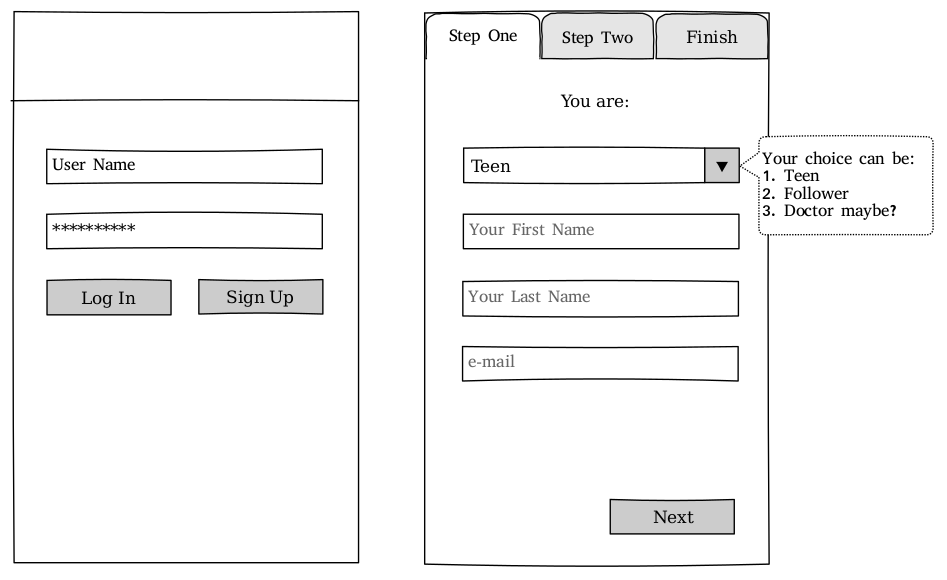
\includegraphics[width=\textwidth,height=\textheight,keepaspectratio]{auth.png}
        \caption{authentication screens}
        \label{fig:screen_auth}
    \end{figure}

    \begin{description}
        \item[Log In] \hfill \\
            The user needs to enter their user name (or e-mail) and password. After hitting on the \emph{Log In} button the app will display the \emph{Check-In} screen (see the figure \ref{fig:screen_checkin}).
        \item[Sign Up] \hfill \\
            The registration process includes several steps, each of which gathers various user's information. Depending on the user type (\emph{Teen} or \emph{Follower}), the information gathered might differ. The \emph{Teen} account will at least include a first name, a last name, a date of birth, and a medical record number. A \emph{Followers} account will probably only include a first and a last name.
            \footnote{Functional Description and App Requirement \#1: The \emph{Teen} is the primary user of the mobile app and is represented in the app by a unit of data containing the core set of identifying information about a diabetic adolescent, including (but not necessarily limited to) a first name, a last name, a date of birth, and a medical record number.}
            Both account types will require an e-mail address.
        \item[Log Out] \hfill \\
            As you can see in the figure \ref{fig:screen_main}, the user can also log out if, for example, another person needs to use the app under their own account.
            \footnote{Basic Project Requirement \#1: App supports multiple users via individual user accounts}
    \end{description}

\newpage

    \subsection{Main Menu}

    To give the users ability to easily navigate between all the screens, the application uses a navigation drawer, which is called \emph{Main Menu}.
    
    Some menu items will indicated additional informations, for example, the number of unseen feedback, unread messages etc.

    \begin{figure}[h]
        \centering
        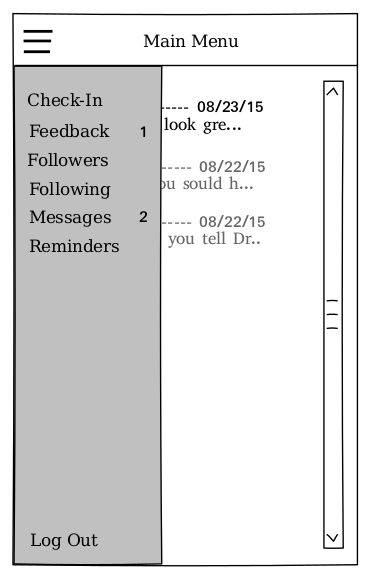
\includegraphics[width=0.5\textwidth,height=\textheight,keepaspectratio]{main.png}
        \caption{main menu}
        \label{fig:screen_main}
    \end{figure}


    This menu and the screens, which can be navigated to from the \emph{Main Menu}, are only available to authenticated users.
    \footnote{Basic Project Requirement \#2: App contains at least one user facing function available only to authenticated users}

\newpage

    \subsection{Check-In}

    This is the main screen for gathering a teen's diabetes related information. It might be open when the user clicks on a check-in notification or be navigated to from the \emph{Main Menu}. The figure \ref{fig:screen_checkin} shows what information will probably be required from a \emph{Teen} user.
    \footnote{Functional Description and App Requirement \#3: Once the \emph{Teen} acknowledges a Reminder, the app opens for a Check-In.  A Check-In includes data associated with that \emph{Teen}, a date, a time, and the user's responses to a set of Questions at that date and time.}

    \begin{figure}[h]
        \centering
        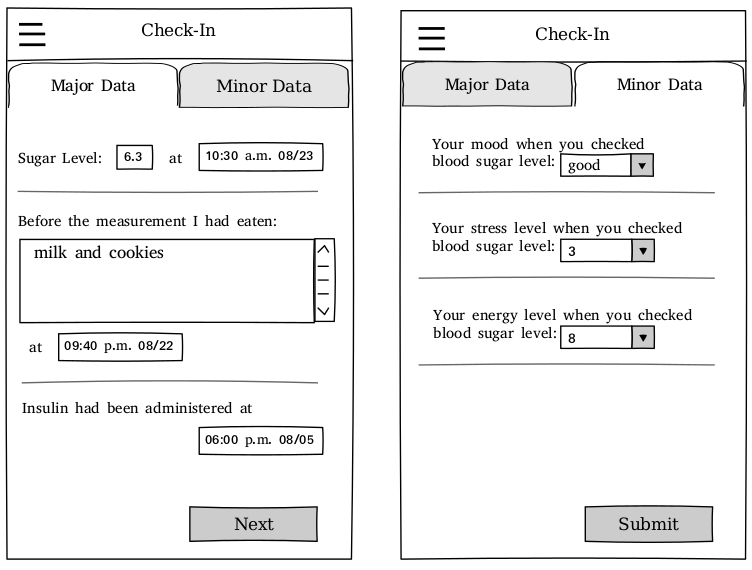
\includegraphics[width=\textwidth,height=\textheight,keepaspectratio]{checkin.png}
        \caption{check-in screen}
        \label{fig:screen_checkin}
    \end{figure}

    This screen is only available for the \emph{Teen} users. The \emph{Follower} users cannot preform check-in's.
    \footnote{Functional Description and App Requirement \#5: The app includes a \emph{Follower} role that is a different type of user (e.g., a parent, clinician, friend, etc.) who does not the ability to perform Check-Ins, but who can receive Check-In data shared from one or more \emph{Teens}. Also, the app allows a \emph{Teen} to be a \emph{Follower} for other \emph{Teens}.}

\newpage

    \subsection{Feedback}

    Both \emph{Teen} and \emph{Follower} accounts can receive feedback from the users they follow. This information will be displayed on the \emph{Feedback} screen (see the figure \ref{fig:screen_feedback}).
    
    Either the \emph{Followers} screen (figure \ref{fig:screen_followers}) or the \emph{Main Menu} (in case of a \emph{Teen} account to see their own feedback data) can be used to navigate to the \emph{Feedback} screen. 

    \begin{figure}[h]
        \centering
        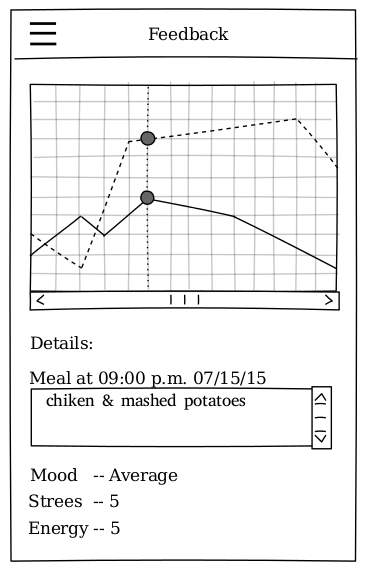
\includegraphics[width=0.5\textwidth,height=\textheight,keepaspectratio]{feedback.png}
        \caption{feedback screen}
        \label{fig:screen_feedback}
    \end{figure}
    
    Whenever a \emph{Teen} submits check-in data, his/her followers will receive feedback via system notifications and/or notifications in the \emph{Main Menu}. 
    \footnote{Functional Description and App Requirement \#4: A \emph{Teen} is able to monitor their feedback data that is updated at some appropriate interval (e.g., when a Check-In is completed, daily, weekly, or when requested by \emph{Followers}). The Feedback data can be viewed graphically on the mobile device.}

    The amount of information will depend on the permissions the corresponding \emph{Teen} granted to their \emph{Follower(s)} (see the figures \ref{fig:screen_followers} and \ref{fig:screen_follow_req}). Additionally, touch gestures will be used to zoom in and zoom out the feedback plot.
    \footnote{Basic Project Requirement \#7: App uses at least one advanced capability or API from the following list: multimedia capture, multimedia playback, touch gestures, sensors, animation.}

\newpage

    \subsection{Followers}

    Each \emph{Teen} account user can have followers. These are users that receive feedback from the \emph{Teen} and can send him/her messages.

    \begin{figure}[h]
        \centering
        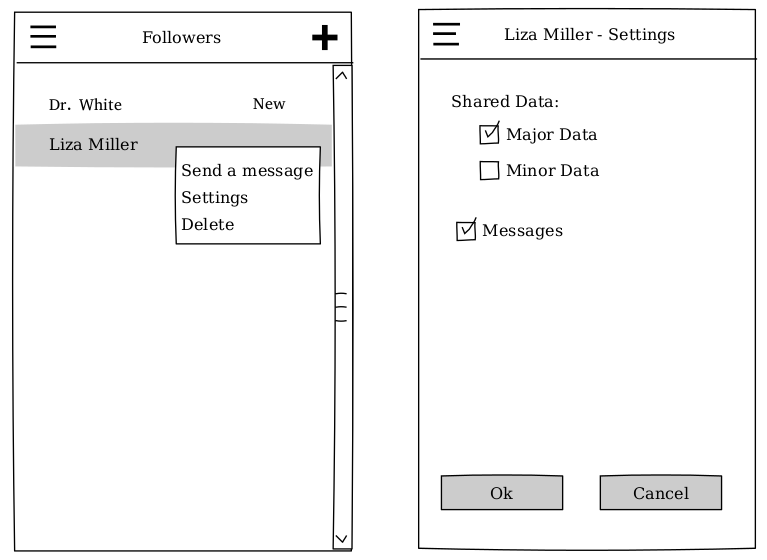
\includegraphics[width=\textwidth,height=\textheight,keepaspectratio]{followers.png}
        \caption{follower and settings screens}
        \label{fig:screen_followers}
    \end{figure}

    As you can see in the figure \ref{fig:screen_followers}, a \emph{Teen} can also change the amount of data he/she wants to share with a certain \emph{Follower}.
    \footnote{Functional Description and App Requirement \#6: The app allows a \emph{Teen} to choose what part(s) of their data to share with one or more \emph{Followers}.}

\newpage

In case if the \emph{Teen} has a new follower request, he/she can click on the corresponding item in the list (figure \ref{fig:screen_followers}) to open the \emph{New Follow Request} screen. The \emph{Teen} can  either accept or reject the request (see the figure \ref{fig:screen_follow_req}).
    
    If the \emph{Teen} wants to invite a \emph{Follower}, the \textbf{+} button can be used to open the corresponding screen, where the \emph{Teen} needs to enter the e-mail the person has used during the registration.
    \footnote{Functional Description and App Requirement \#7: The app only allows \emph{Teen} data to be disseminated to authorized/authenticated \emph{Followers} and accessed over HTTPS to enhance privacy and security of the data (the HTTPS part will be described in the implementation details)}
    The person, whom the invite has been sent to, will receive a notification where he/she can accept/reject the invitation.

    \begin{figure}[h]
        \centering
        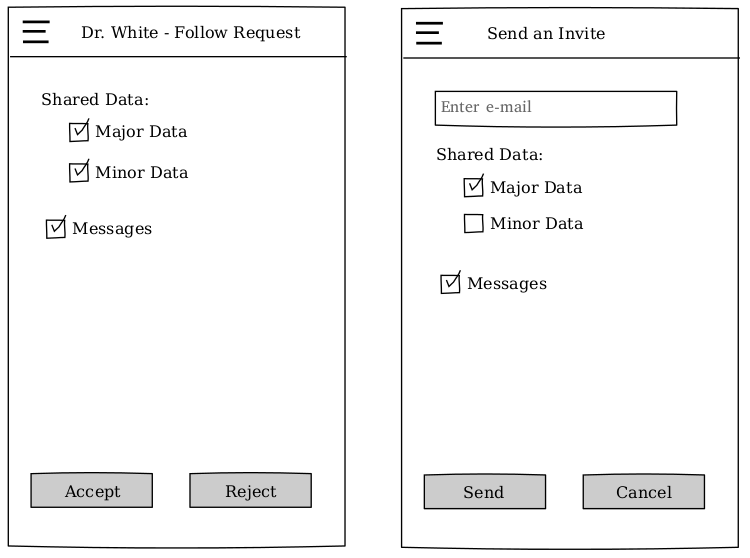
\includegraphics[width=\textwidth,height=\textheight,keepaspectratio]{follow_req.png}
        \caption{follow request and invitation screens}
        \label{fig:screen_follow_req}
    \end{figure}

\newpage

    \subsection{Following}

    To see the list of the users you currently follow the \emph{Following} screen can be used. The user can access feedback of the users he/she follows or start to follow another one by clicking on the \textbf{+} button (see the figure \ref{fig:screen_following}).

    \begin{figure}[h]
        \centering
        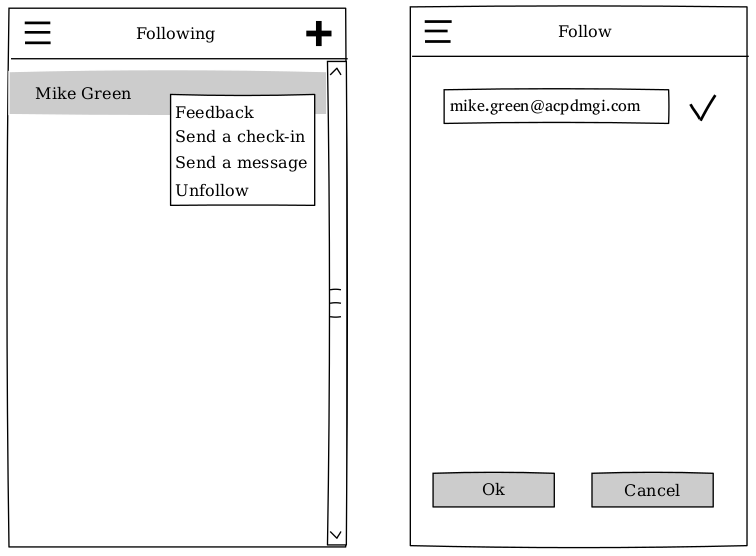
\includegraphics[width=\textwidth,height=\textheight,keepaspectratio]{following.png}
        \caption{following screen}
        \label{fig:screen_following}
    \end{figure}

\newpage

    \subsection{Reminders}

    Each \emph{Teen} will receive check-in reminders in the form of alarms at least three times a day. Once a reminder has been received a \emph{Teen} can tap on the notification and the \emph{Check-In} screen will be open to perform the check-in process.
    Reminder can be added, edited or tuned on/off  using the \emph{Reminders} screen (see the figure \ref{fig:screen_reminders}). At least three reminders will always be on.
    \footnote{Functional Description and App Requirement \#2: The \emph{Teen} receives a Reminder in the form of alarms or notifications at patient-adjustable times at least three times per day.}

    \begin{figure}[h]
        \centering
        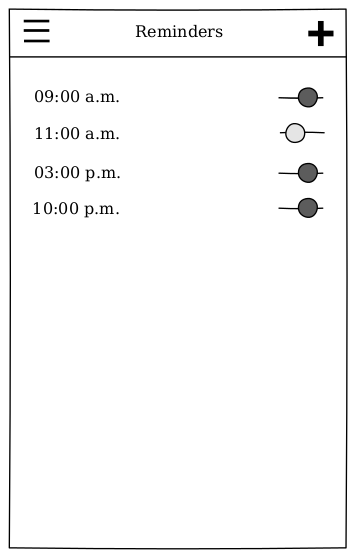
\includegraphics[width=0.5\textwidth,height=\textheight,keepaspectratio]{reminders.png}
        \caption{reminders screen}
        \label{fig:screen_reminders}
    \end{figure}

\newpage

    \subsection{Optional Features}

    The following features will be implemented only if the major capstone project requirements are met and there is development time left.

    \begin{itemize}
        \item Messages

            \emph{Teen} account will be able to communicate with their \emph{Followers} and vice versa by using the \emph{Messages} screen. A \emph{Teen} or their \emph{Follower(s)} will be able to communicate in the form of a dialog (see the figure \ref{fig:screen_messages}).


            \begin{figure}[h]
                \centering
                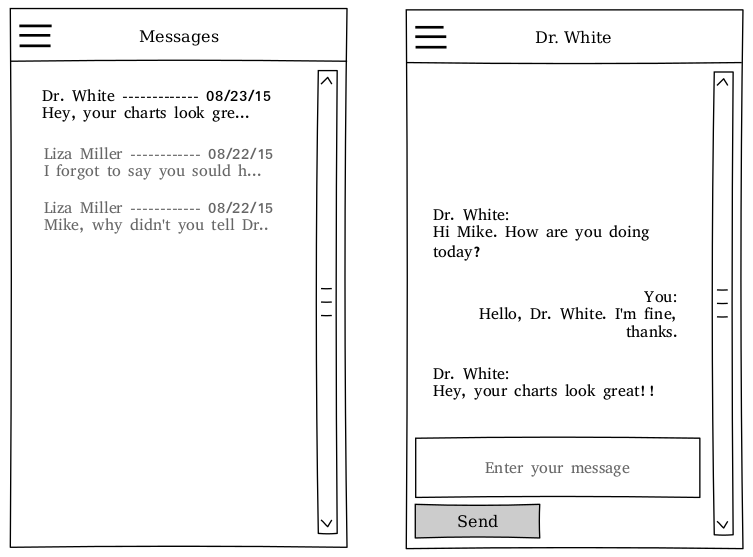
\includegraphics[width=\textwidth,height=\textheight,keepaspectratio]{messages.png}
                \caption{messages and dialog screens}
                \label{fig:screen_messages}
            \end{figure}

        \item User Settings (the screen is not present)
    \end{itemize}
            This screen will allow to alter different user information and settings. For example, a user could change the password or turn some notifications off.

\newpage

\section{Implementation Details}

This section describes the implementation details of the application's components at a very high level. There will be provided an example of use of some of those components to give you a picture of how they are going to interact.

\newpage

    \subsection{Client and Server Side Implementation}
    
    \begin{description}
        \item[Client Side] \hfill \\
            The client side is represented by an android-based application.
        \item[Server Side] \hfill \\
            The server side of the project is represented by a remotely-hosted Java Spring-based service.
            \footnote{Basic Project Requirement \#4: App interacts with at least one remotely-hosted Java Spring-based service} 
            For the sake of simplicity and due to the lack of time, no scaling capabilities is going to be used.
    \end{description}

    \subsection{Security}

    \begin{description}
        \item[Client-Server Communication] \hfill \\
            All network communication between the client and server side is done via HTTPS.
            \footnote{Basic Project Requirement \#5: App interacts over the network via HTTP/HTTPS}
            For test purposes the project uses a self-signed SSL certificate, which should be changed in production. The client side is distributed with the public-key certificate, which is stored inside a JKS keystore in resources/raw. 
        \item[User Security] \hfill \\
            OAuth2 is used for the user authorization. All interactions with the client (except for the \emph{Authentication} screen) and the server can be done only if an access token has been granted to the user. Once an access token has been received, it is saved into shared preferences on the client side, so that it can be used from any place in the application and the user could use the app when the network is off (for example, to work with the cached feedback).
        \item[User Credentials Security] \hfill \\
            The users passwords are not stored on the server side. Instead of the plain text format, hash value and salt is used to verify the users credentials.
    \end{description}

    \subsection{Data Management}

    \begin{description}
        \item[Client Side] \hfill \\
            The activities and fragments will be as stateless as possible and hold almost no data in order to facilitate configuration changes. A content provider backed by an SQL database will be used to store cached server data, so that this data could be used even if the user is off-line.
        \item[Server Side] \hfill \\
            The server uses a separate MySQL database to store all the users' data.
    \end{description}

    \subsection{Network Operations}

    \begin{description}
        \item[Client Side] \hfill \\
        All client side network operations will be performed in a background thread via a single intent service.
        \footnote{Basic Project Requirement \#8: App supports at least one operation that is performed off the UI Thread in one or more background Threads or Thread pool.}
        Once the intent service has received data from the server, it hands it over to the intermediate service (the data is received via a local broadcast receiver) and waits for another network request from the activities/fragments.
        
        The intermediate service delivers data to the content provider. After the content provider's data has been updated, the corresponding loader will update the activity/fragment based on the changes in the content provider. This will separate logic and data and will make it easy to handle configurations changes.
        \footnote{Basic Project Requirement \#3: App comprises at least 1 instance of each of at least 2 of the following 4 fundamental Android components: Activity, BroadcastReceiver, Service, ContentProvider}
        \item[Server Side] \hfill \\
            The server network operation will be performed via a google cloud messaging server. The GCM server will then deliver any updates to the corresponding client by using push notifications. Depending on the type of the info from the server, a push notification will contain either entire data or ``command'' for the client side (for example, to fetch new feedback from the server).
    \end{description}

    \subsection{Client GUI}

    As you could see in the ``User-Facing Components'' section, the client side GUI will be represented by at least 10 screens.
    \footnote{Basic Project Requirement \#6: App allows users to navigate between 3 or more user interface screens at runtime}
    Those screen will most likely be implemented using 2-3 activities and 7-8 fragments. The use of fragments should make the GUI smoother and make it easier to re-use pieces of the user interface.

\newpage

    \subsection{Example Components' Usage}

    This is an example of how the certain components are used when one user sends a follow request to another user. Just follow the arrows to see in what order the parts are being used during request.

    \begin{figure}[ht]
         \centering
         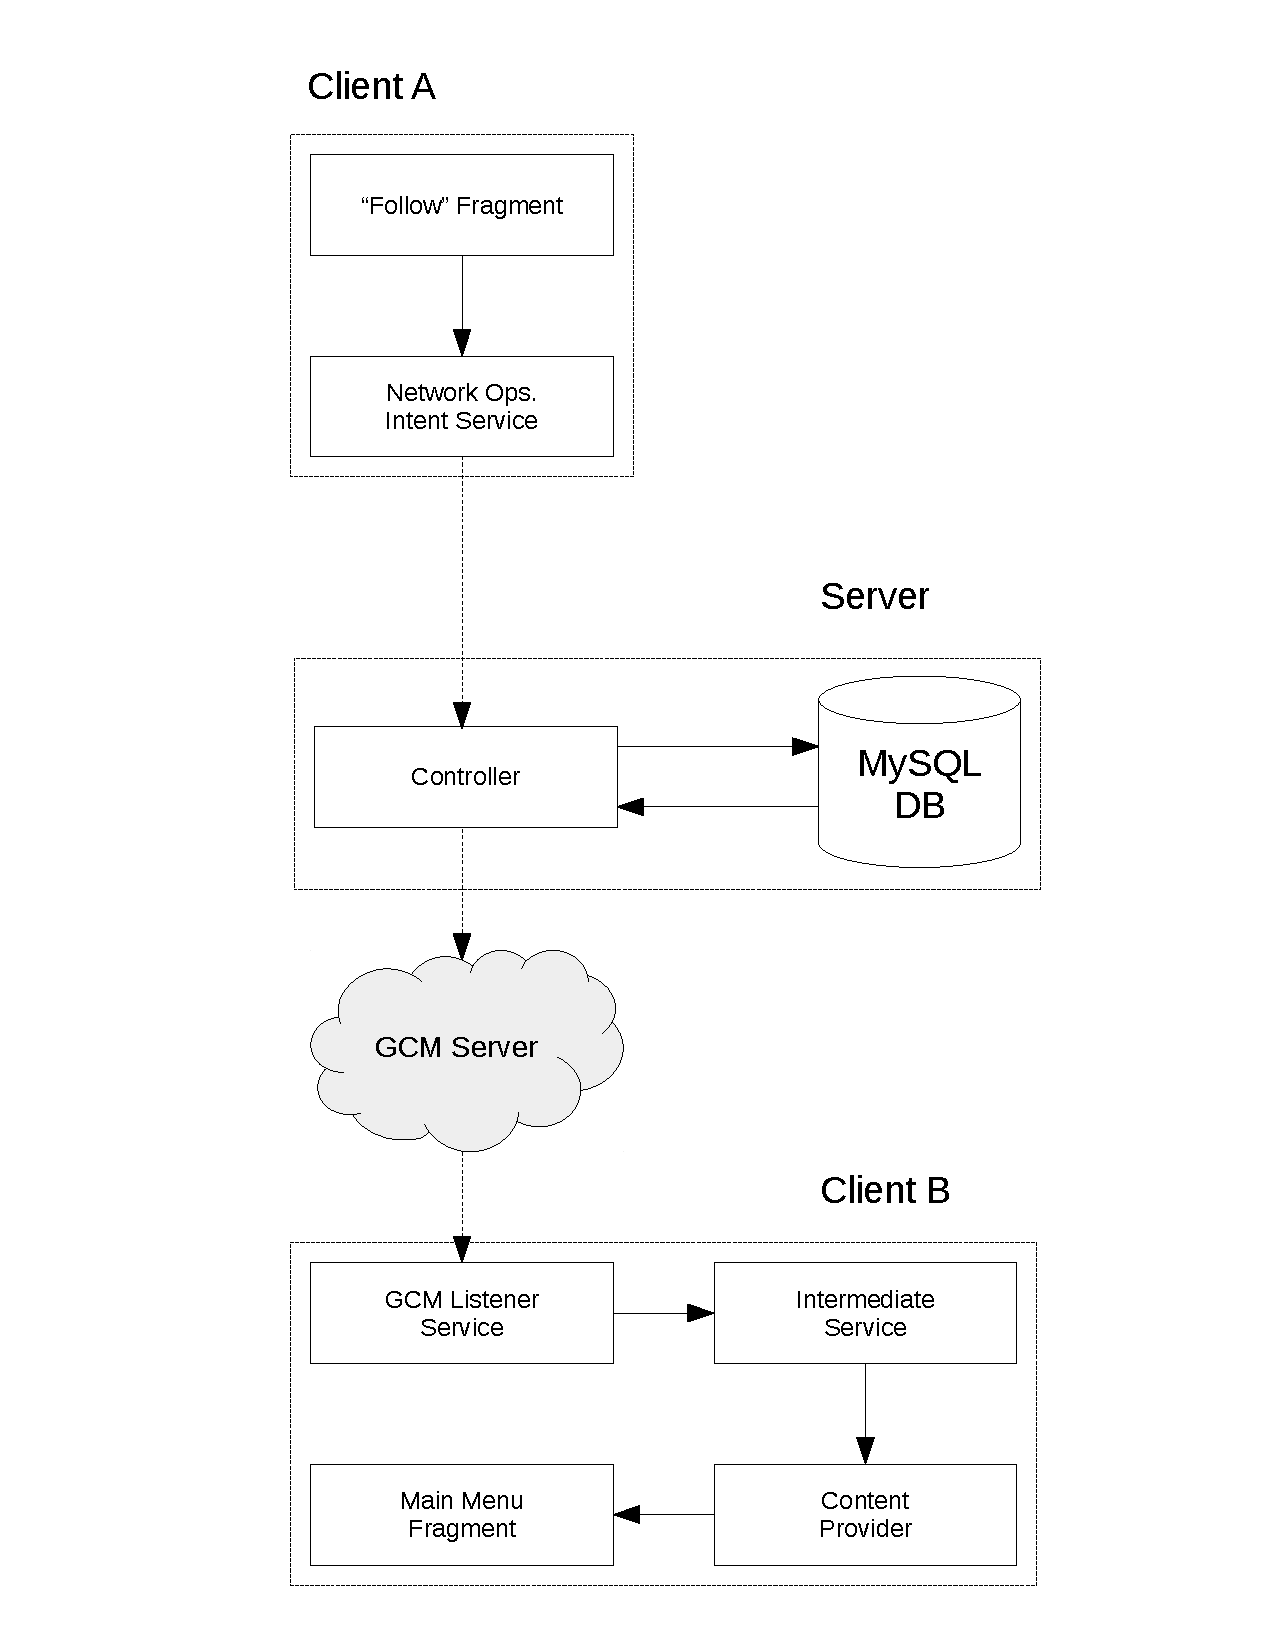
\includegraphics[page=1,width=\textwidth,height=0.7\textheight,keepaspectratio]{follow_req_workflow.pdf}
         \caption{follow request workflow}
         \label{fig:screen_follow_req_workflow}
    \end{figure}

\newpage
\pagenumbering{gobble}

\clearpage
\vspace*{\fill}
\begin{center}
    \begin{minipage}{0.4\textwidth}
        \fontsize{28}{12}\selectfont
        Thank You!
    \end{minipage}
\end{center}
\vfill
\clearpage

\end{document}
